\documentclass{article}

\usepackage[utf8]{inputenc}
\usepackage{cancel}
\usepackage{amsmath, amssymb, amsfonts}
\usepackage[binary-units]{siunitx}
\usepackage{tikz}
\usepackage{float}
\usepackage{pgffor}
\usepackage{import}
\usepackage{vwcol}
\usepackage{fontawesome}
\usepackage{stmaryrd}
\usepackage{multicol}
\usepackage{pdfpages}
\usepackage{transparent}
\usepackage{xcolor}
\usepackage{scalerel}
\usepackage{stackengine}
\usepackage{algpseudocode}
\newcommand{\diag}{\operatorname{diag}}
\newcommand{\card}{\operatorname{card}}
\newcommand{\tr}{\operatorname{tr}}
\newcommand{\rg}{\operatorname{rg}}
\renewcommand{\epsilon}{\varepsilon}
\newcommand{\equivalent}[1]{\underset{#1}{\sim}}
\newcommand{\R}{\mathbb{R}}
\newcommand{\Q}{\mathbb{Q}}
\newcommand{\C}{\mathbb{C}}
\newcommand{\N}{\mathbb{N}}
\newcommand{\Z}{\mathbb{Z}}
\newcommand{\cM}{\mathcal{M}}
\newcommand{\cO}{\mathcal{O}}
\newcommand{\dx}{\mathrm{d}x}
\newcommand{\dy}{\mathrm{d}y}
\newcommand{\dz}{\mathrm{d}z}
\newcommand{\dt}{\mathrm{d}t}
\newcommand{\df}{\mathrm{d}f}
\newcommand{\Sp}{\operatorname{Sp}}
\newcommand{\dangersign}[1][2ex]{%
  \renewcommand\stacktype{L}%
  \scaleto{\stackon[1.3pt]{\color{red}$\triangle$}{\tiny !}}{#1}%
}

\usepackage[a4paper,top=4cm,bottom=4cm,left=3cm,right=3cm,marginparwidth=1.75cm]{geometry}
% \newcommand{\incfig}[2][1]{%
%     \def\svgwidth{#1\columnwidth}
%     \import{./figures/}{#2.pdf_tex}
% }
% 
\newenvironment{theorem}[1][\unskip]{
	\paragraph{Théorème #1}

}{}

\newenvironment{proof}[1][\unskip]{
	\def\temp{#1}\ifx\temp\empty
		\paragraph{Preuve}
	\else
		\paragraph{Preuve \emph{(#1)}}
	\fi

}{}

\newenvironment{definition}[1][\unskip]{
	\paragraph{Définition: #1}

}{}

\newenvironment{warning}[1][\unskip]
{
	\vspace{1cm}
	\begin{minipage}[c]{0.1\linewidth}
	\dangersign[8ex] 
\end{minipage}%
\begin{minipage}[l]{0.9\linewidth}
}
{
	\end{minipage}
	\vspace{1cm}
}

% \pdfsuppresswarningpagegroup=1

\usepackage{minted}
\usepackage{url}
\setcounter{tocdepth}{1}

\begin{document}
    \title{
        
\includegraphics[width=0.5\textwidth]{logo-enseeiht.png}
        \\[3cm]
        Proposition de sujets \\
        Projet long \\
        UE Technologie objet
    }

    \author{Alexandre Trotel, Ayoub Bouchama, Clément Cognard, \\
    Ewen Le Bihan, Florent Puy, Gauthier Rancoule, Raphaël Giudice}
    \date{12 Février 2023}

    \maketitle
    \tableofcontents

    \newpage

    \section{Interface graphique pour \emph{ortfo} }
    \paragraph{}
    
    \emph{ortfo}  (\url{https://github.com/ortfo}) est un système de génération de sites portfolio à partir de
fichiers de descriptions stockés à même les dossiers des projets figurant dans ce portfolio, ce qui
simplifie grandement l’organisation pour l’utilisateur.

\paragraph{}

Cependant, écrire ce fichier de description demande une certaine aisance technique: c’est
un fichier de texte brut écrit en markdown, avec une syntaxe particulièrement complexe pour
l’utilisateur lambda pour décrire l’agencement des différents blocs de contenu (par exemple, avoir
un paragraphe et une image côte-à-côte):

    \begin{minted}[fontsize=\footnotesize]{markdown}
---
tag: [cli, program, app, gui, web]
made with: [go, svelte, json, yaml, markdown]
layout: [[intro], [why], [description], [description_example, database, database_example]]
started: 2020-06-26
---

# ortfo

:: fr

@intro
Un système de génération de portfolios faits maison.

@why
Ayant un grand nombres de projets (plus de 200), il me fallait une solution permettant de facilement 
les ajouter à mon portfolio. Je voulais un système qui me permette d'avoir l'entrée dans mon portfolio 
d'un projet stockée avec le projet lui même, dans le même dossier, par soucis d'organisation. Je voulais 
également un site totalement généré, car il en résulterait un site très rapide et plus facile à maintenir.

@description
## ortfo/db
J'ai eu l'idée de stocker l'entrée portfolio d'un projet dans un sous-dossier `.portfoliodb` à l'intérieur 
du dossier du projet, d'y décrire chaque projet avec du [markdown](/using/markdown).
Ensuite, il y a 3 types de blocs: des paragraphes, des liens isolés (utiles pour mettre en valeur un lien 
vers le site réalisé ou le code source, par exemple) et des médias (vidéos, images, PDFs, etc.).
On peut également, avec une extension syntaxique sur mesure, traduire les articles en plusieurs langues

@description_example
![](./description_example.md "Un exemple de fichier de description de portfolio")

@database
Après, ces entrées sont collectées et mises en commun dans un fichier [JSON](/using/json) constituant la 
base de donéee du portfolio: c'est la partie 'db' de ortfo

@database_example
![](./database_example.json "Une base de donnée après analyse des différents fichiers markdown")
    \end{minted}

L'application permettrait à l'utilisateur de gérer la création automatique de ces fichiers à partir d'une interface graphique basée sur des blocs, de gérer:

\begin{itemize}
    \item L'édition des métadonnées du projet (date de création, tags, technologies utilisées, etc.)
    \item L'écriture du contenu de l'entrée dans des blocs de contenu
    \item La traduction du contenu dans plusieurs langues
    \item L'ajout de médias (images, vidéos, etc.)
    \item L'agencement en colonnes des blocs en glissant et déposant (à la \emph{Elementor}, \emph{Wix}, etc.)
    \item L'exportation et publication du site en un clic
\end{itemize}

\newpage

\section{Reg7}

Un logiciel d'analyse et de construction d'expressions rationelles depuis une interface intuitive.

Le but serait de permettre l'écriture d'exprsesions rationelles complexes de manière simple et visuelle.

La partie analyse existe déjà sous forme de site web, le site \url{https://regexr.com}:

\begin{figure}[H]
    \centering
    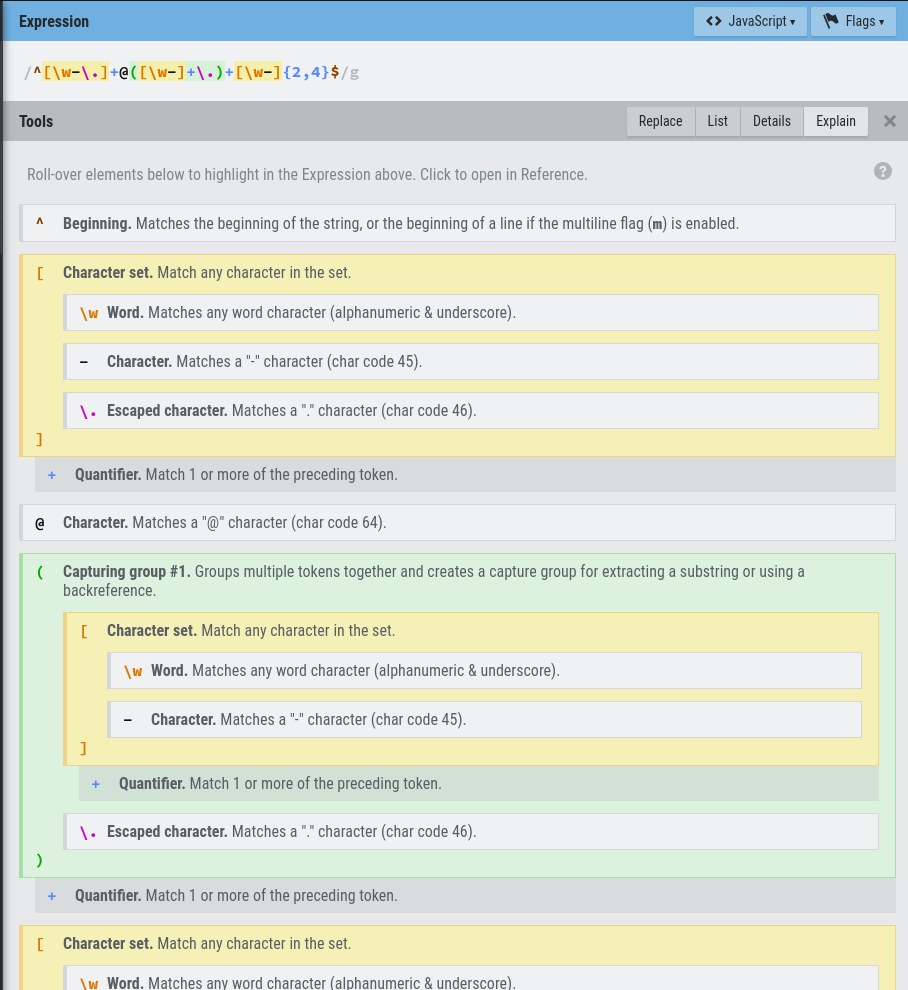
\includegraphics[width=0.8\textwidth]{regexr.com.png}
    \caption{Interface du site regex}
    \label{fig:reg7:regexr}
\end{figure}

Cette logique en blocs imbriqués (à la \emph{Scratch}) pourra être utilisée pour composer des expressions rationnelles, en plus de l'analyse d'expressions existantes.

Le logiciel proposera:

\begin{itemize}
    \item L'importation d'expressions régulières
    \item Un pannel de différents blocs (un bloc ``set de caractères", un bloc ``groupe de capture", etc).
    \item L'exportation en différentes ``saveurs" d'expressions régulières (Perl, Vim, etc.) 
    \item Un champ de texte permettant de tester son expression sur des valeurs concrètes
\end{itemize}

\section{Moteur de rendu}
Le but est de créer un moteur de rendu qui prend une carte 2D en entrée, génère la représentation 3D du monde et permet à l'utilisateur  d'explorer avec différentes perspectives et angles.

\subsection{Caractéristiques}
Le moteur de rendu 3D aura les caractéristiques suivantes :

\begin{description}
    \item[Visualisation 3D]  Les utilisateurs peuvent naviguer dans le monde 3D.
    \item[Éclairage] Le monde 3D pourra être éclairé à l'aide de sources de lumières.
    \item[Ombres] Des ombres seront projetées par les objets et les murs.
    \item[Réflexions] Les surfaces réfléchissantes seront incluses .
    \item[Textures] Des textures pourront être appliquées
    \item[Paramètres personnalisables] L'utilisateur aura la possibilité de régler divers paramètres tels que l'éclairage, les ombres, les reflets et les textures.
\end{description}

\paragraph{}

Les utilisateurs peuvent utiliser le moteur de rendu de deux manières différentes

\begin{description}
    \item[En utilisant une image] Les utilisateurs peuvent utiliser une image qui représente la carte 2D dans le logiciel. Cette image sera traitée par le logiciel, qui extraira les informations sur les murs, les objets et les autres éléments de la carte depuis l'image en lisant les pixels. 
    \item[Saisie directe depuis le logiciel] Les utilisateurs peuvent également saisir la carte directement dans le logiciel en créant la carte en 2D à l'aide d'outils de dessin pour les murs, les objets et d'autres éléments. 
\end{description}

\subsection{Fonctionnement}
Le rendu sera principalement fait à partir de raytracing qui permettra de calculer l'affichage des murs et des objects sur le point de vu de l'utlisateur.

\subsection{Résultat attendu}
Le résultat final de ce projet sera un moteur de rendu 3D qui peut générer des mondes 3D à partir d'une carte 2D en utilisant du raycasting. Le moteur de rendu offrira une expérience réaliste et immersive aux utilisateurs.

\newpage
\section{Tabless}

Un nouveau type de navigateur web sans onglets.

L'idée est d'arrêter d'avoir beaucoup d'onglets ouverts et de devoir les fermer au bout d'une demi-heure d'inutilité, ou de crouler sous les plus de cents onglets ouverts.

À la place, les concepts d'historique, d'onglets et de pages à voir plus tard sont fusionnées en une pile appelée \emph{The Stack}.

Ainsi, les onglets deviennent les sites ouverts actuellement (partie \emph{Actuellement}), qui passent automatiquement dans la partie historique au bout d'un certain temps, et les sites à visiter plus tard passent naturellement dans la partie \emph{Actuellement} à leur ouverture.

\begin{figure}[H]
    \centering
    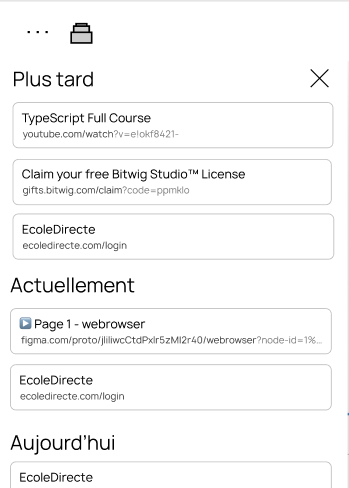
\includegraphics[width=0.5\textwidth]{tabless.png}
    \caption{Concept de \emph{The Stack}}
    \label{fig:tabless}
\end{figure}
    

Le logiciel devra proposer les fonctionnalités suivantes

\begin{itemize}
    \item Navigation vers un site depuis la barre d'adresse-recherche avec suggestions
    \item Mode ``immersif" où les quelques éléments d'interface prennent le moins de place possible pour laisser le site prendre le plus de place possible de la fenêtre
    \item Gestion de préférences de l'utilisateur (moteur de recherche utilisé, thème clair/sombre)
    \item Gestion intelligente des téléchargements: emplacements de sauvegarde différents selon le type de fichier, le domaine et le titre de l'onglet
    \item \emph{The Stack} (fonctionnalité expliquée précédemment)
    \item Support d'extensions Chrome
\end{itemize}

\end{document}
